\documentclass{article}

\usepackage{graphicx}
\usepackage{tikz}
\usepackage{tikzsymbols}
\usetikzlibrary{calc,patterns,shapes.geometric}
\pagestyle{empty}
\usepackage[margin=0pt]{geometry}
\geometry{papersize={14in,12in}}

\def\centerarc[#1](#2)(#3:#4:#5){\draw[#1] ($(#2)+({#5*cos(#3)},{#5*sin(#3)})$) arc (#3:#4:#5);}

\begin{document}
	\begin{figure}
		\centering
		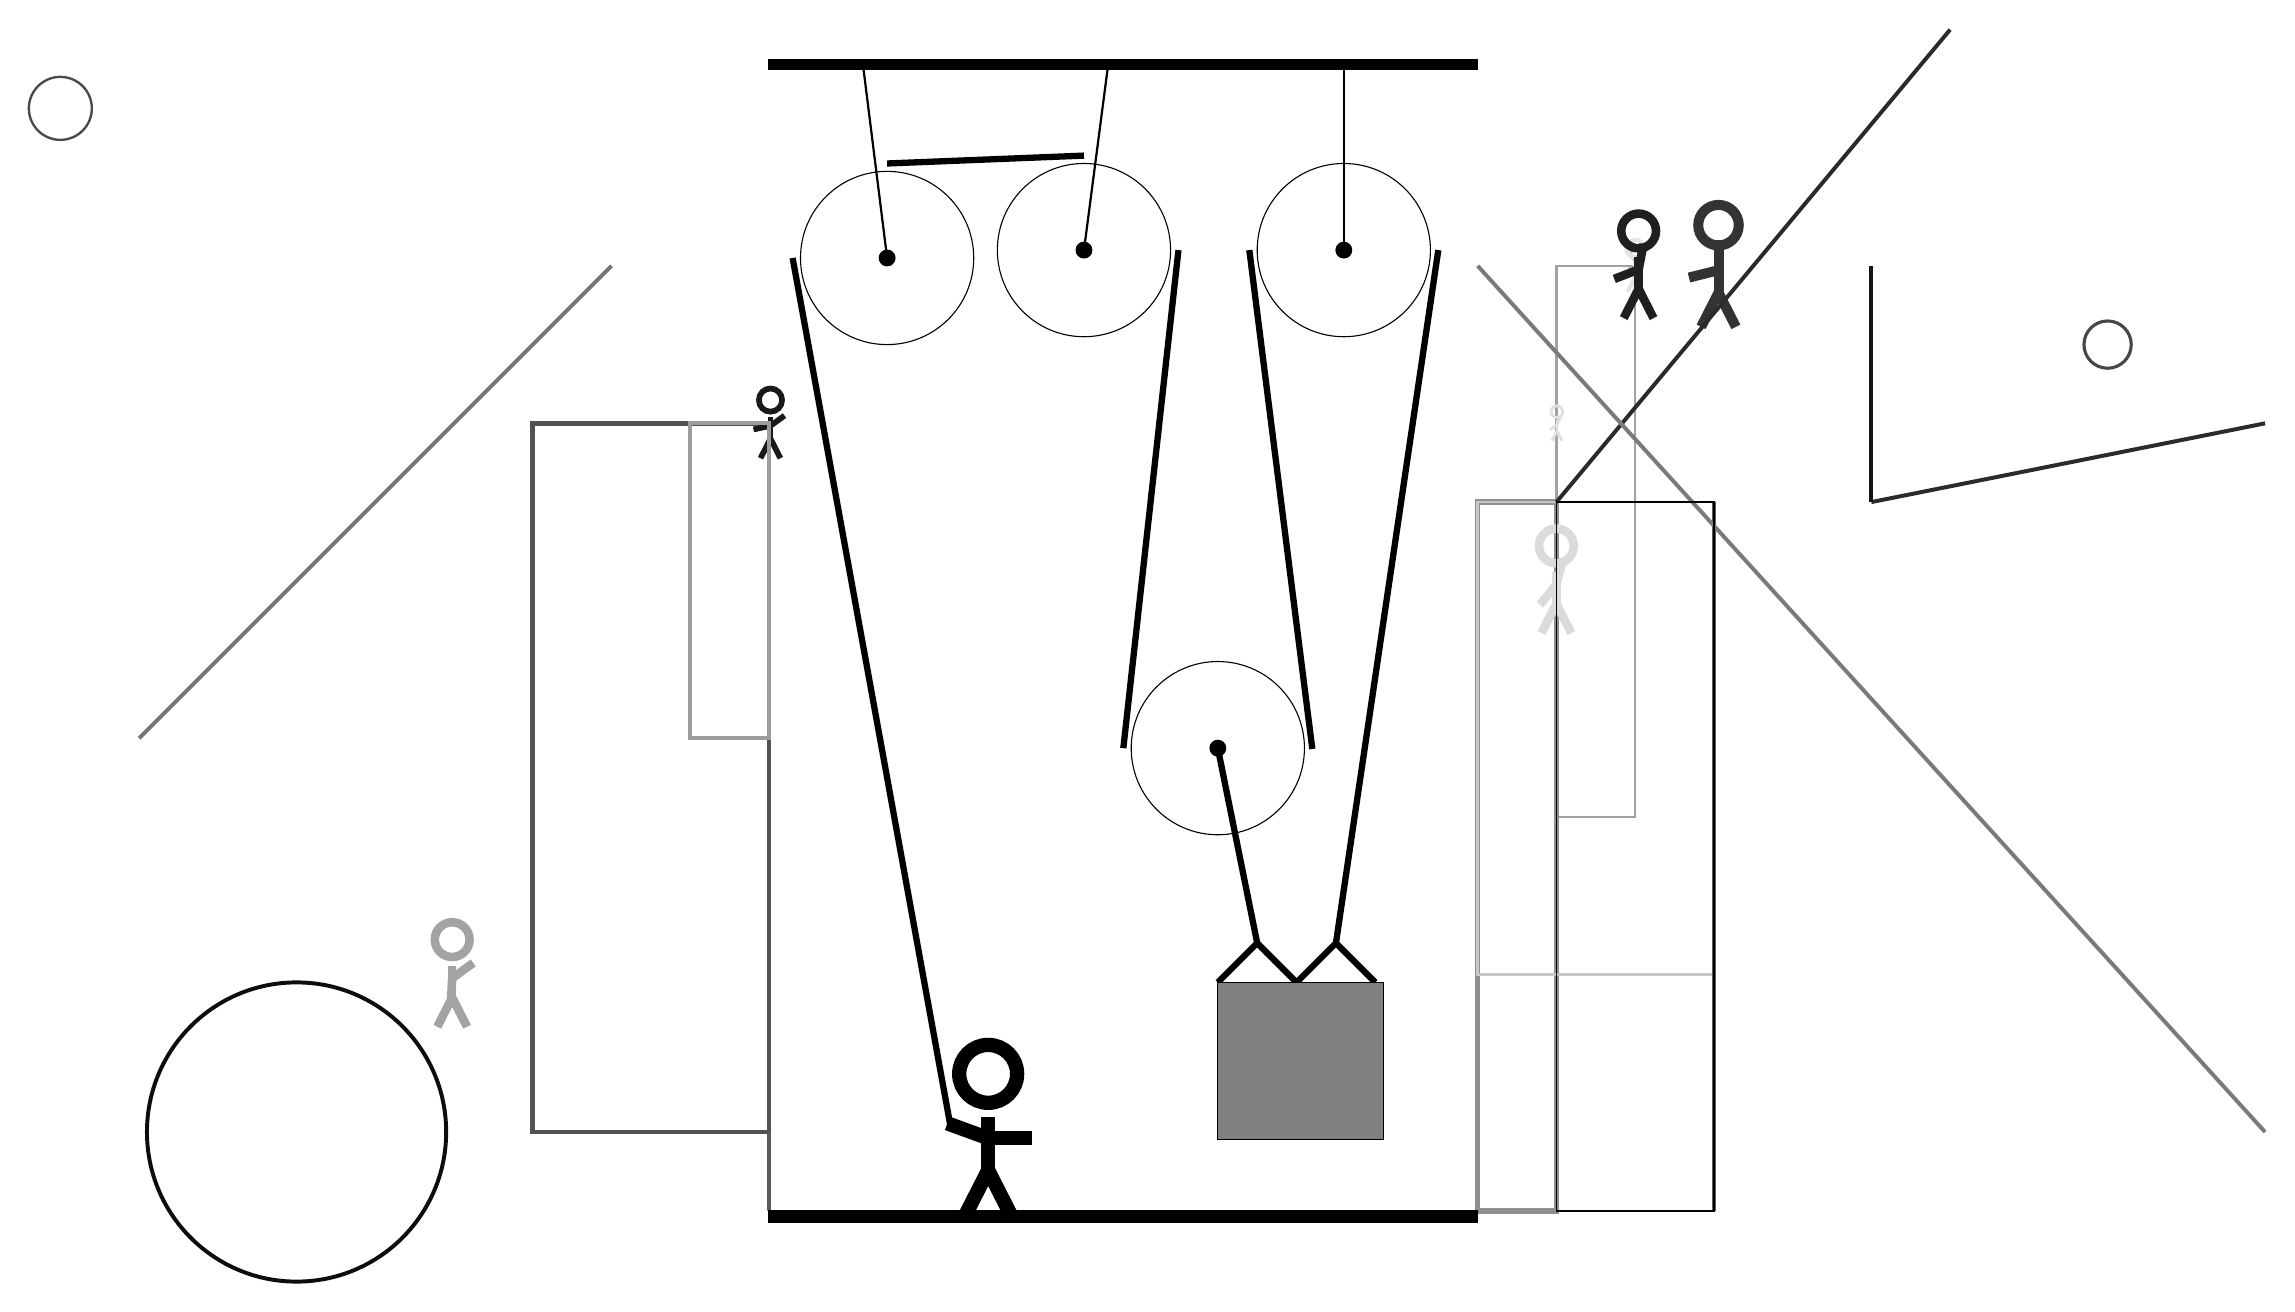
\begin{tikzpicture}
			%%%%% START %%%%%
			
			\draw[fill=black] (-3, 11.5) rectangle (6, 11.625);
			
			\draw (1, 9.2) circle (1.1);
			\draw[fill=black] (1, 9.2) circle (0.1);
			\draw[thick] (1, 9.2) -- (1.3, 11.5);
			
			\draw (4.3, 9.2) circle (1.1);
			\draw[fill=black] (4.3, 9.2) circle (0.1);
			\draw[thick] (4.3, 9.2) -- (4.3, 11.5);
			
			\draw (2.7, 2.875) circle (1.1);
			\draw[fill=black] (2.7, 2.875) circle (0.1);
			
			\node[line width=0.5mm, color=black!36] at (-7, 0) {\Strichmaxerl[6][87][36]};
			
			\draw[line width=0.6mm, color=black!68] (-3, -2) rectangle (-6, 7);
			\node[line width=0.4mm, color=black!24] at (8, 9) {\Strichmaxerl[2][3][55]};
			\draw[line width=0.3mm, color=black!37] (7, 2) rectangle (8, 9);
			
			\draw [line width=0.3mm, color=black!71](-12, 11) circle (0.4);
			\draw[line width=0.7mm, color=black!44] (7, -3) rectangle (6, 6);
			\draw[line width=0.5mm, color=black!54](-5, 9) -- (-11, 3);
			\draw[line width=0.5mm, color=black!65] (-3, -2) rectangle (-3, -3);
			\draw[line width=0.3mm, color=black!22] (6, 6) rectangle (9, 0);
			\draw[line width=0.5mm, color=black!83](11, 6) -- (16, 7);
			
			\node[line width=0.2mm, color=black!90] at (-3, 7) {\Strichmaxerl[4][12][36]};
			
			\draw [line width=0.4mm, color=black!72](14, 8) circle (0.3);
			\node[line width=0.4mm, color=black!80] at (9, 9) {\Strichmaxerl[7][14][90]};
			
			\draw[line width=0.5mm, color=black!39] (-3, 7) rectangle (-4, 3);
			\draw[line width=0.5mm, color=black!83](7, 6) -- (12, 12);
			\draw[line width=0.5mm, color=black!63](9, 6) -- (9, -3);
			\draw [line width=0.5mm, color=black!95](-9, -2) circle (1.9);
			\node[line width=0.3mm, color=black!10] at (8, 9) {\Strichmaxerl[3][89][69]};
			\node[line width=0.7mm, color=black!14] at (7, 5) {\Strichmaxerl[6][51][75]};
			
			\draw[line width=0.5mm, color=black!52](6, 9) -- (16, -2);
			\draw[line width=0.2mm, color=black!100] (7, 6) rectangle (9, -3);
			
			\draw[line width=0.5mm, color=black!92](11, 6) -- (11, 9);
			
			\node[line width=0.4mm, color=black!88] at (8, 9) {\Strichmaxerl[6][21][79]};
			\node[line width=0.7mm, color=black!12] at (7, 7) {\Strichmaxerl[2][37][64]};
			
			\draw[line width=0.8mm]  (2.7, -0.1) -- (3.2, 0.4) -- (3.7, -0.1) -- (4.2, 0.4) -- (4.7, -0.1);
			\draw[fill=black!50] (2.7, -0.1) rectangle (4.8, -2.1);
			
			\draw (-1.5, 9.1) circle (1.1);
			\draw[fill=black] (-1.5, 9.1) circle (0.1);
			\draw[thick] (-1.5, 9.1) -- (-1.8, 11.5);
			
			\draw[line width=0.8mm](-0.7, -1.9) --  (-2.7, 9.1);
			\centerarc[line width=0.8mm](-1.5, 9.1)(90:180:1.2000000000000002);
			\draw[line width=0.8mm](-1.5, 10.3) -- (1, 10.4);
			\centerarc[line width=0.8mm](1, 9.2)(0:90:1.2000000000000002);
			\draw[line width=0.8mm](2.2, 9.2) -- (1.5, 2.875);
			\centerarc[line width=0.8mm](2.7, 2.875)(180:370:1.2000000000000002);
			\draw[line width=0.8mm] (3.9, 2.865) -- (3.1, 9.2);
			\centerarc[line width=0.8mm](4.3, 9.2)(0:180:1.2000000000000002);
			\draw[line width=0.8mm](4.2, 0.4) -- (5.5, 9.2);
			\draw[line width=0.8mm] (3.2, 0.4) -- (2.7, 2.875);
			
			\node at (-0.2, -2) {\Strichmaxerl[10][-20][0]};
			
			\draw[fill=black] (-3, -3) rectangle (6, -3.15);
			
			%%%%% END %%%%%
		\end{tikzpicture}
	\end{figure}	
\end{document}